\section{Тестирование}

\subsection{Условия тестирования}

\begin{itemize}
	\item{Процессор: AMD Ryzen 5 4600H, 3.00 ГГц}
	\item{Оперативная память: 16 ГБ, DDR4}
	\item{Операционная система: Windows 10}
	\item{IDE: Visual Studio 2022 17.5, версия компилятора: 19.35.32216.1}
	\item{Усредненные результаты по 10 запускам на каждом шаге}
\end{itemize}

\subsection{Результаты тестирования}

Результаты эксперимента 1. Время работы алгоритма Грэхема в зависимости от количества точек во входных данных.

\begin{figure}[h]
	\centering
	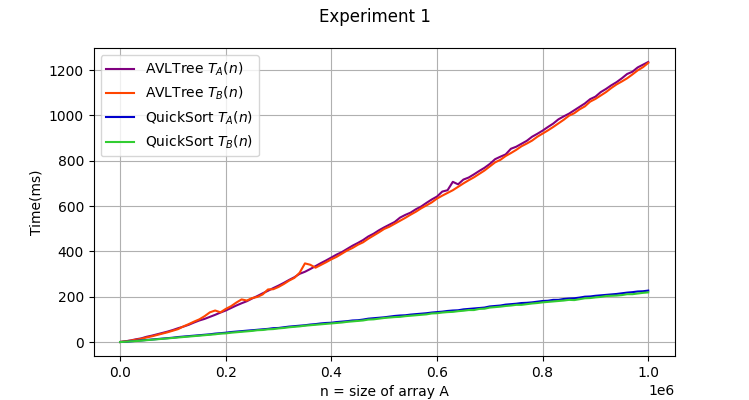
\includegraphics[width=\textwidth]{Images/Experiment_1.png}
	\caption{Эксперимент 1 ($E1$)}
	\label{fig:experiment_1}
\end{figure}

\newpage

Результаты эксперимента 2. Время работы алгоритма Грэхема в зависимости от размера квадрата, в который вписаны случайные точки из входного множества.

\begin{figure}[h]
	\centering
	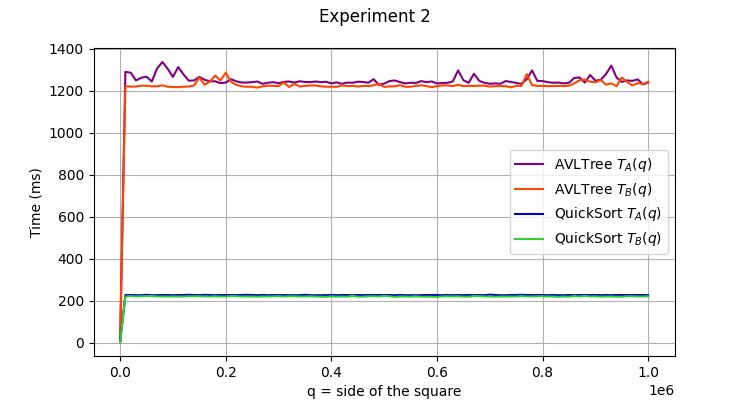
\includegraphics[width=\textwidth]{Images/Experiment_2.png}
	\caption{Эксперимент 2 ($E2$)}
	\label{fig:experiment_2}
\end{figure}

\newpage